\chapter{Neuronové sítě}
Neuronové sítě (Neural Network)~\cite{link1}~\cite{link20} jsou výpočetní modely inspirované komplexním systémem přenosů informací v biologickém mozku.
Základními stavebními jednotkami výpočetního modelu neuronové sítě jsou neurony, které mají své vstupy, váhy a výstup.

Každý neuron obdrží vstupní data od jiných neuronů, přičemž každému vstupu je předána určitá váha.
Váhy slouží k určení důležitosti jednotlivých vstupů.
Neuron zpracovává své vstupní data pomocí aktivačních funkcí a provede souhrn vážených vstupů.
Výsledek této operace je pak předán dalším neuronům jako výstup.

Je důležité poznamenat, že neuronový model~\ref{fig:Model neuronu} může mít libovolný počet vstupů a vah, ale každý neuron generuje pouze jeden výstup.
Tímto způsobem se vytváří komplexní sítě neuronů, které spolupracují při zpracování informací a řešení problémů.

Neuronové sítě se využívají v mnoha oblastech umělé inteligence a strojového učení.
Jejich schopnost zpracovávat složité vzorce a adaptovat se na data je důležitá pro úspěšné řešení rozmanitých úloh, jako je rozpoznávání obrazu, překlad textu, predikce a další.

\begin{figure}[H]
	\centering
	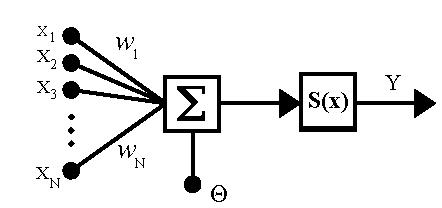
\includegraphics[width=0.6\textwidth]{Figures/NeuronModel.jpg}
	\caption{Model neuronu~\cite{link1}}\label{fig:Model neuronu}
\end{figure}

V následujícím vzorci je formule podle McCulloch–Pitts modelu neuronu.
Váhy se zde násobí společně se vstupními daty, které se následně sčítají a upravují podle parametrizované hodnoty tzv.\ biasu.
Výsledek se vkládá do aktivační funkce a vychází výstup, který se posílá na vstup následujícímu neuronu.

\[Y = S(\sum_{i=1}^{N}(W_{i} X_{i}) + \Theta)\]

\begin{itemize}
\item $X$: vstupní data
\item $W$: váhy mezi neurony
\item $\Theta$: threshold obvykle pod jménem bias
\item $S(x)$: aktivační funkce
\item $Y$: výstup neuronu
\end{itemize}
Proces, při kterém se vstupní data postupně předávají z jednoho neuronu na druhý až k výstupu, se nazývá dopředná propagace (forward propagation).

Při dopředné propagaci se vstupní data předají do prvního neuronu, který provede výpočet pomocí aktivační funkce a vah a výsledek předá jako výstup druhému neuronu.
Tento proces se opakuje, dokud výstup nedorazí ke konečnému neuronu nebo výstupní vrstvě neuronové sítě.

\section{Učení neuronové sítě}
Cílem neuronové sítě je optimalizovat své váhy a biasy tak, aby dosahovala co nejlepších výsledků na základě trénovacích dat.
Trénovací data jsou data, která slouží k učení a nastavení parametrů sítě tak, aby byla schopna správně predikovat výstupy pro nová, dosud neviděná data.

Proces trénování neuronové sítě obecně probíhá ve třech fázích:

Dopředná propagace (Forward propagation): Vstupní data jsou předána sítí, která je pomocí vah a biasů upravuje a předává z neuronu na neuron až k výstupní vrstvě.
V této fázi se vypočítávají aktivační funkce a výstupy jednotlivých neuronů.

Zpětná propagace (Backward propagation): Po provedení dopředné propagace se porovnávají výstupy sítě s očekávanými výstupy na základě trénovacích dat.
Mezi těmito výstupy je chyba propagována zpět skrze síť a jsou vypočítány gradienty, které udávají směr a míru, pomocí jaké je potřeba upravit váhy a biasy jednotlivých neuronů.
    
Aktualizace vah: Na základě gradientů zpětné propagace jsou aktualizovány váhy a biasy neuronů, aby byly přizpůsobeny tak a minimalizovaly tak chybu mezi výstupy sítě a očekávanými výstupy.
Tím se zlepšuje schopnost sítě predikovat správné výstupy.

Tento proces trénování se opakuje pro každou trénovací sadu dat, aby se síť co nejlépe přizpůsobila dané úloze.
Cílem je dosáhnout co nejnižší chyby na trénovacích datech a zároveň dosáhnout schopnosti generalizovat a správně predikovat výstupy i pro nová, dosud neviděná data (testovací či provozní data).

\subsection{Učení pod dohledem}
Při trénování pod dohledem (supervised) neuronové sítě jsou použita trénovací data jako vzor, na základě kterého je pomocí aktuálních nastavení vah a biasů vypočten výstup sítě viz.~dopředná propagace.
Tento výstup je následně porovnán s požadovaným výstupem a vypočtena chyba, která udává rozdíl mezi predikovaným a očekávaným výstupem viz.~zpětná propagace.

\subsection{Volné učení}
Volné učení (unsupervised) je typ učení, kde trénovací data nejsou doprovázena předem danými a chtěnými výstupy.
Na rozdíl od učení pod dohledem (supervised), kde jsou k dispozici páry vstupů s požadovanými výstupy, učení bez dohledu se snaží najít vzorce, struktury nebo skryté informace ve vstupních datech samotných.

Při učení bez dohledu je modelu předloženo pouze množství neoznačených trénovacích dat.
Cílem je objevit struktury, shluky, vzory nebo jiné charakteristiky v datech, aniž by byly předem specifikovány.
Model se učí tím, že přizpůsobuje své váhy a biasy tak, aby optimalizoval určité cílové kriterium, jako je minimalizace chyby nebo maximalizace pravděpodobnosti dat.

\section{Rekurentní neuronové sítě}
Rekurentní neuronové sítě (Recurrent neural network -~RNN)~\cite{link16} jsou architekturou neuronových sítí, která je navržena speciálně pro práci se sekvenčními daty.
Sekvenčními daty se rozumí data, která mají určitý časový nebo prostorový kontext a jsou uspořádána ve formě sekvence nebo posloupnosti.

Hlavním rysem RNN je schopnost uchovávat vnitřní stav (hidden state) a předávat ho ze vstupní vrstvy do následujících časových kroků.
To znamená, že RNN může zpracovávat a modelovat závislosti a vztahy mezi jednotlivými prvky v sekvenci.

V kontextu sekvencí je RNN schopna zohlednit předchozí vstupy a stav sítě a použít je k výpočtu aktuálního výstupu.
Tím je RNN efektivní pro úkoly, jako je předpovídání dalšího prvku v sekvenci (např.\ predikce dalšího slova ve větě), překlad sekvenčních dat (jako je strojový překlad) nebo analýza sentimentu v textu.

\subsection{Zjednodušeně popsané fungování rekurentní neuronové sítě}
Rekurentní neuronová síť (RNN) pracuje se sekvencemi dat.
V případě věty `Já jsem člověk' by se postupně vkládala jednotlivá slova do sítě a RNN by vytvářela výstupy na základě předchozích informací.

Na začátku sekvence je slovo `Já', které se vloží do sítě, a RNN generuje odpovídající výstup.
Poté se slovo `jsem' spolu s informací z předchozího kroku (výstupem zpracování slova `Já') vkládá do sítě a RNN generuje nový výstup.
Tímto způsobem se postupně zpracovávají všechna slova v sekvenci.

Důležité je, že RNN udržuje vnitřní stav, který slouží k předávání informace mezi jednotlivými časovými kroky.
Při zpracování slova `jsem' se do vstupu RNN přidá i informace z předchozího kroku, která obsahuje informaci o slově `Já'.
Tímto způsobem se RNN postupně `paměťově' obohacuje o předchozí informace.

Na konci sekvence má RNN teoreticky informace o všech předchozích slovech, protože se vnitřní stav přenáší z jednoho kroku na druhý.
Tato schopnost zachytit kontext a závislosti mezi slovy v sekvenci je předností RNN a umožňuje tím efektivně pracovat se sekvenčními daty.

\subsection{Architektura rekurentních neuronových sítí}
Architektura rekurentní neuronové sítě~\ref{fig:RNN architektura} jednoho neuronu vypadá následovně.

\begin{figure}[H]
	\centering
	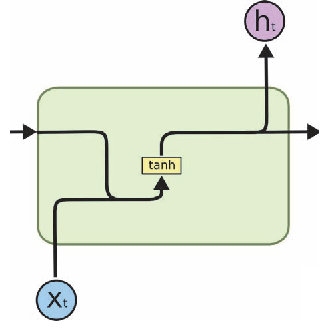
\includegraphics[width=0.3\textwidth]{Figures/RNN_basic_architecture.png}
	\caption{RNN architektura~\cite{link2}}\label{fig:RNN architektura}
\end{figure}

Neuron v rekurentní neuronové síti (RNN) sdílí některé vlastnosti s neurony v běžné neuronové síti.
Do neuronu RNN přicházejí vstupní data ze současného kroku (aktuální vstup) a také data z předchozích kroků (vnitřní stav).

Před zpracováním těchto dat se nad nimi provádí aktivační funkce.
Jednou z běžně používaných aktivačních funkcí v RNN je hyperbolický tangens.
Aktivační funkce hyperbolický tangens převádí vstupní hodnoty na rozmezí mezi -1 a 1.

Aktivační funkce hyperbolický tangens, v následujícím vzorci, se často používá v RNN, protože umožňuje zachování informací z předchozích kroků a přenášení těchto informací do dalších výpočtů.
Díky tomu může RNN efektivně zachycovat závislosti na časové ose a pracovat se sekvencemi dat.

\[h_{t} = \tanh(W_{hh} h_{t-1} + W_{xh} x_{t})\]

\subsubsection{Neduhy rekurentních neuronových sítí}
Rekurentní neuronové sítě (RNN) mají problém s dlouhodobými závislostmi a mizejícím gradientem, což omezuje jejich schopnost efektivně zachycovat dlouhodobé informace v sekvencích dat.

Mizející gradient se projevuje tím, že při zpětném šíření chyby se gradient postupně zmenšuje a při trénování se váhy příliš neaktualizují.
To znamená, že dlouhodobé závislosti mezi vstupy v sekvenci se obtížněji přenášejí a RNN nemusí být schopná se naučit efektivně využívat informace z dávnějších kroků.

Long Short-Term Memory (LSTM) a Gated Recurrent Unit (GRU) jsou vylepšené architektury RNN, které byly navrženy právě s cílem řešit tyto problémy.
Tyto modely používají brány, pro kontrolu probíhajících informací v síti.

LSTM obsahuje speciální paměťovou jednotku, která umožňuje uchovávat a aktualizovat informace na základě brán.
Brány umožňují kontrolovat, které informace jsou považovány za důležité a udržovat je v paměti po delší dobu.

Vylepšení GRU je podobné LSTM, ale s jednodušší architekturou.
Obsahuje aktualizační bránu, která rozhoduje, jak moc má být aktualizovaná paměťová jednotka, a resetovací bránu, která rozhoduje, jakou část paměti zapomenout.
Tímto způsobem se GRU snaží efektivně uchovávat a aktualizovat informace o kontextu.

Tyto vylepšené architektury RNN, jako LSTM a GRU, přinášejí zlepšení v schopnosti zachytit dlouhodobé závislosti a lépe uchovávat kontext při práci se sekvencemi dat.

\section{Long Short-Term Memory}
Long Short-Term Memory (LSTM)~\cite{link3} je speciální verzí rekurentní neuronové sítě, která byla představena v roce 1997 Hochreiterem a Schmidhuberem.

LSTM bylo navrženo specificky k řešení problému s dlouhodobou závislostí a pamatováním informací na delší časový úsek.
Jedním z hlavních problémů standardních rekurentních neuronových sítí je, že mají tendenci rychle zapomenout informace z minulých kroků, což omezuje jejich schopnost zachytit dlouhodobé závislosti v datech.

LSTM využívá speciální strukturu paměťové jednotky, která je schopná efektivně uchovávat a aktualizovat informace na základě brán.
Tato struktura umožňuje paměťové jednotce rozhodovat, které informace mají být zapomenuty a které mají být uchovány na delší dobu.

Díky svému návrhu LSTM~\ref{fig:LSTM architektura} umožňuje neuronové síti uchovávat informace o kontextu na delší časový úsek a lépe pracovat s dlouhými sekvencemi dat.
To přispívá k větší efektivitě a schopnosti modelu zachytit vztahy a závislosti v datech na delších časových škálách.

\begin{figure}[H]
	\centering
	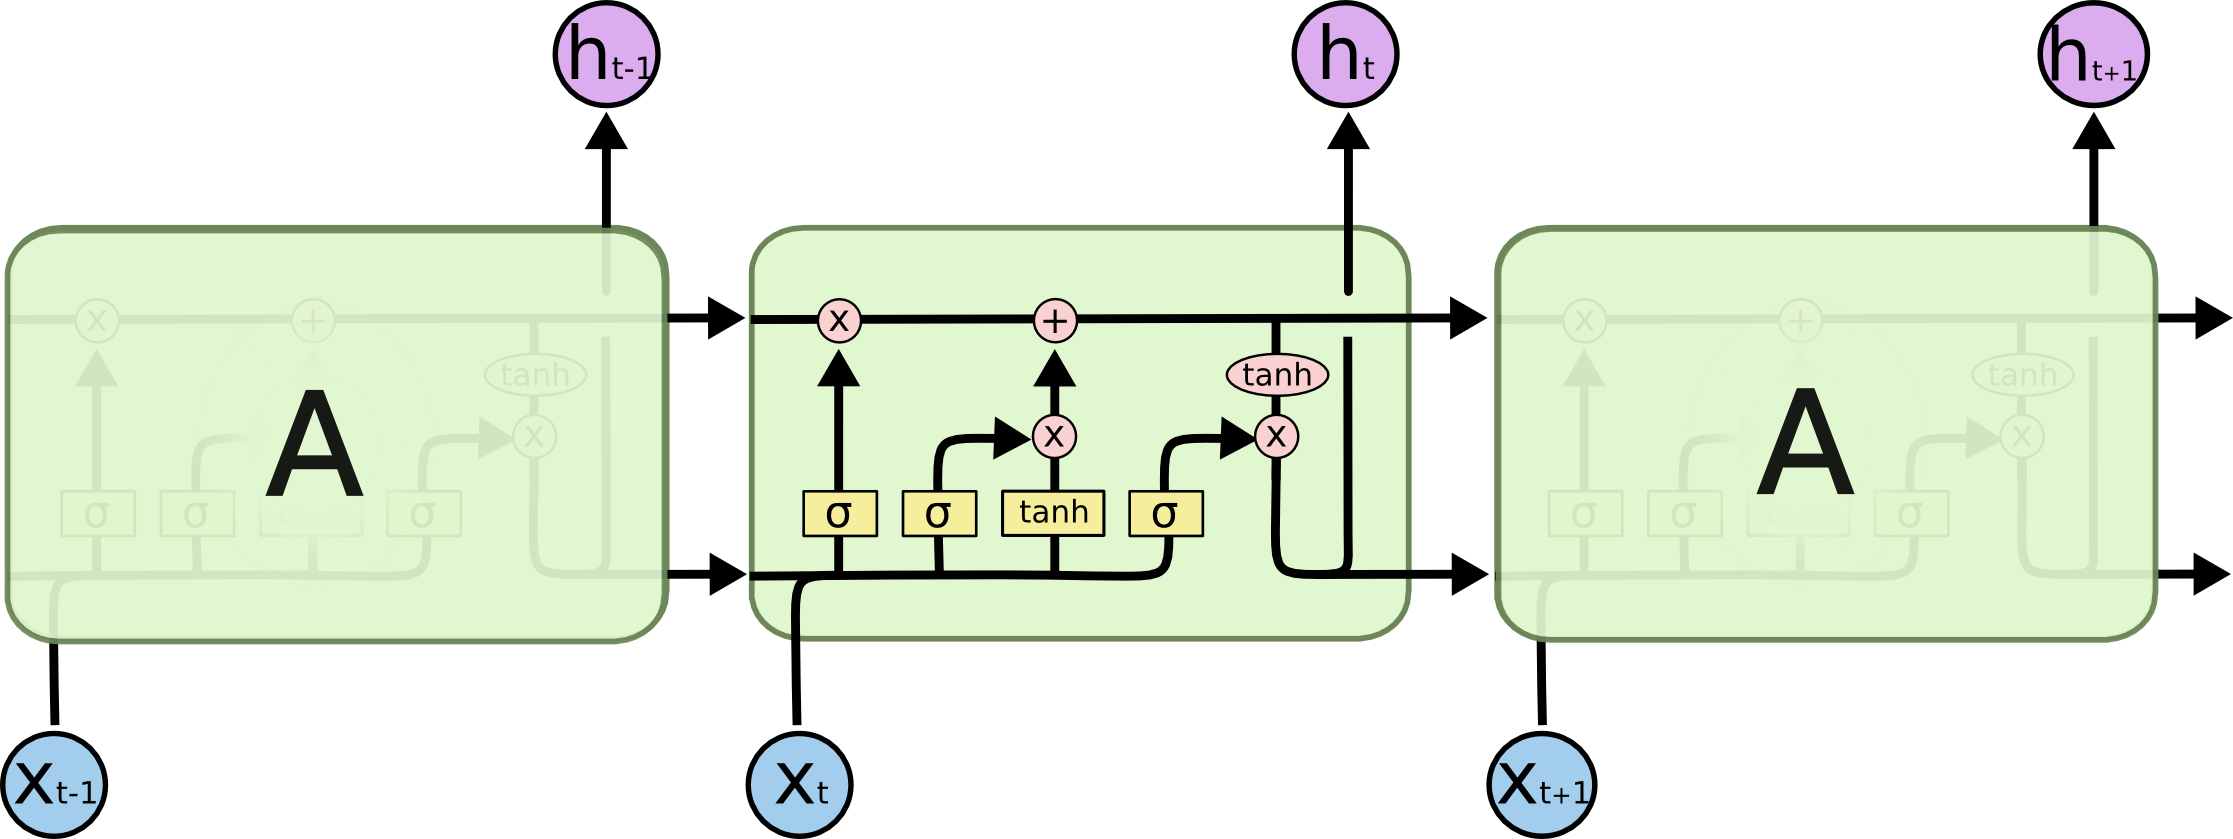
\includegraphics[width=0.8\textwidth]{Figures/LSTM_architecture.png}
	\caption{LSTM architektura~\cite{link3}}\label{fig:LSTM architektura}
\end{figure}

Architektura LSTM je oproti standardní RNN značně komplexnější.
Hlavním rozšířením jsou právě brány~\ref{fig:LSTM architektura neuronu}, které jsou klíčovým prvkem v této architektuře.

\begin{figure}[H]
	\centering
	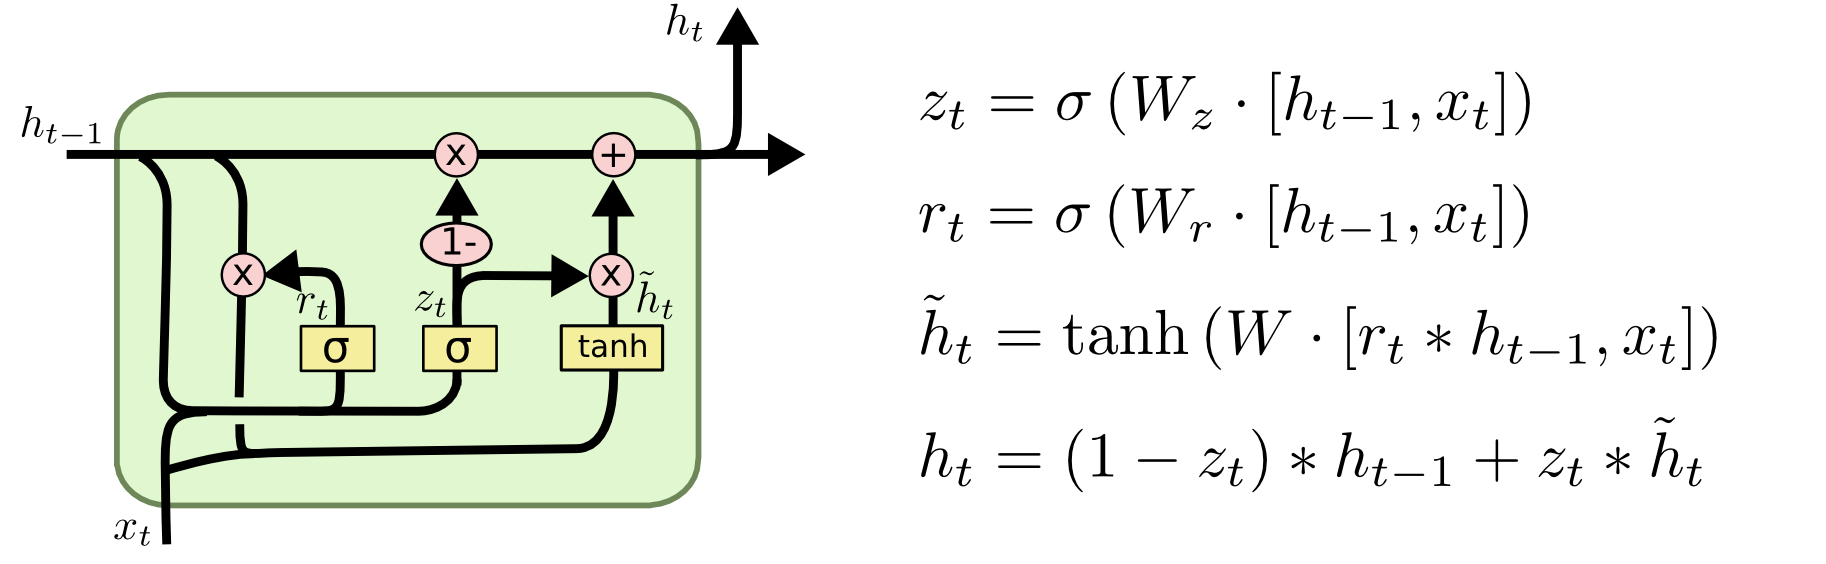
\includegraphics[width=0.8\textwidth]{Figures/LSTM_architecture_neuron.png}
	\caption{LSTM architektura neuronu~\cite{link3}}\label{fig:LSTM architektura neuronu}
\end{figure}

LSTM obsahuje tři základní brány: zapomnětlivou bránu (forget gate), vstupní bránu (input gate) a výstupní bránu (output gate).
Tyto brány spolu s paměťovou jednotkou (memory cell) umožňují LSTM učit se a efektivně pracovat s dlouhodobými závislostmi v datech.
Brány umožňují paměťové jednotce filtrovat a rozhodovat, které informace mají být zapomenuty, které nové informace mají být přidány a které informace mají být využity při výstupu.

\subsection{Zapomnětlivá brána}
Zapomnětlivá brána (forget gate) rozhoduje, jakou část minulého stavu by měl LSTM zapomenout. Na základě vstupů a předchozího stavu určuje, které informace mají být zahozeny.

\subsection{Vstupní brána}
Vstupní brána (input gate) rozhoduje, které nové informace by měly být uloženy v paměťové jednotce LSTM.\@
Pomocí aktivační funkce, využívající sigmoid funkci, určuje, které hodnoty mají být aktualizovány.

\subsection{Výstupní brána}
Výstupní brána (output gate) rozhoduje, jaká část paměťového stavu by měla být odeslána jako výstup z LSTM.\@
Sigmoidová aktivační funkce ovlivňuje, které hodnoty budou výstupem.

\section{Gated Recurrent Unit}
Gated Recurrent Unit (GRU)~\cite{link4} je další speciální verze rekurentní neuronové sítě, která byla představena v roce 2014 Cho et al.
Architektura GRU je navržena k řešení problému mizejícího gradientu, který je běžným problémem standardních RNN.\@

Podobně jako LSTM využívá GRU aktualizační a resetovací brány.
Tyto brány~\ref{fig:GRU architektura neuronu}~\ref{fig:GRU vyznam operaci} umožňují GRU učit se zachovávat informace z dřívějších kroků.
GRU se snaží efektivně zpracovávat dlouhodobé závislosti a současně snižovat problém mizejícího gradientu.

\begin{figure}[H]
	\centering
	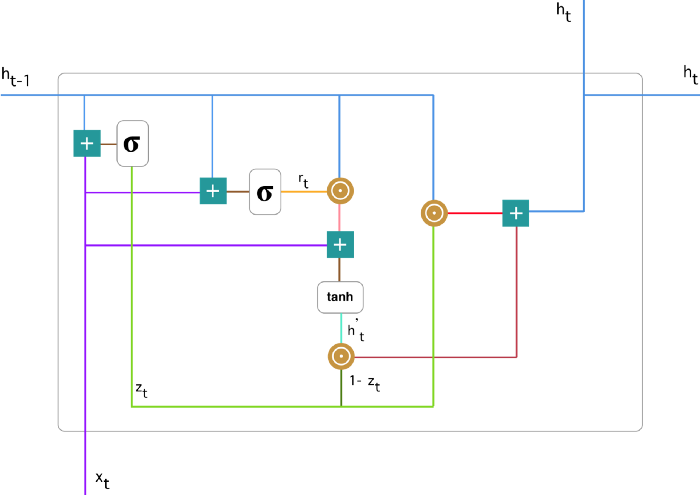
\includegraphics[width=0.8\textwidth]{Figures/GRU_architecture_neuron.png}
	\caption{GRU architektura neuronu~\cite{link4}}\label{fig:GRU architektura neuronu}
\end{figure}

\begin{figure}[H]
	\centering
	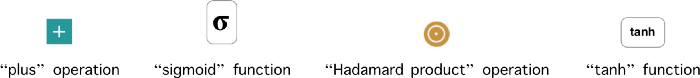
\includegraphics[width=0.8\textwidth]{Figures/GRU_math_operation.png}
	\caption{GRU význam operací~\cite{link4}}\label{fig:GRU vyznam operaci}
\end{figure}

\subsection{Aktualizační brána}
Aktualizační brána (update gate) rozhoduje, jakou část minulého stavu by měla být aktualizována a která část by měla zůstat nezměněna.
Brána pomocí sigmoidové aktivační funkce určuje, jakou část informací z minulého stavu si GRU ponechá a jakou část upraví.

\[z_{t} = \sigma(W^{(z)} x_{t} + U^{(z)} h_{t-1})\]

\subsection{Resetovací brána}
Resetovací brána (reset gate) rozhoduje, jakým způsobem se budou kombinovat vstupní data s předchozím stavem.
Opět pomocí sigmoidové aktivační funkce určuje, které informace se mají resetovat a které se mají zapomenout.

\[r_{t} = \sigma(W^{(r)} x_{t} + U^{(r)} h_{t-1})\]

\subsection{Porovnání}
Vzhledem k popisu problému, jak rozhodnout, zda je text přeložen strojem nebo napsán člověkem, je vhodné využít RNN, konkrétně LSTM a GRU, které jsou navrženy pro zpracování sekvencí dat a řeší problémy původních RNN.\@

LSTM a GRU jsou obě vylepšené architektury RNN, které se snaží překonat problém mizejícího gradientu a zachovat dlouhodobé závislosti v sekvencích.
Oba modely mají některé podobné prvky a často dosahují podobných výsledků.
Obě architektury se liší v počtu a funkcionalitě brán a každá má své výhody.

LSTM je považováno za komplexnější a má větší počet parametrů k učení.
Je navrženo tak, aby si pamatovalo informace z dlouhodobých závislostí a je schopno lépe zachovávat kontext v delších sekvencích.

Na druhou stranu GRU je jednodušší a má menší počet parametrů.
Architektura je navržena tak, aby byla rychlejší a efektivnější v učení.
Je vhodnější pro scénáře, kde je omezený počet trénovacích dat nebo kde je důležitá výpočetní efektivita.
\endinput